\documentclass[]{scrreprt}
\usepackage{amsmath,amsfonts,graphicx}
\usepackage{multirow}
\usepackage{pslatex}
\usepackage{tabularx}
\usepackage{comment}
\usepackage{xspace}
\usepackage{array}

\usepackage{hyperref}

\usepackage{caption}
\DeclareCaptionFont{white}{\color{white}}
\DeclareCaptionFormat{listing}{\colorbox{gray}{\parbox{\textwidth}{#1#2#3}}}

\graphicspath{
{figures/}
}

\def\species{\mathrm{sp}}
\def\phase{\mathrm{ph}}
\def\massfrac{\chi}
\def\flux{\mathbf{F}}
\def\darcyvel{\mathbf{v}}
\def\energydens{\mathcal{E}}
\def\d{\mathrm{d}}

\newcommand{\uo}{\mbox{UO\textsubscript{2}}\xspace}

\setcounter{secnumdepth}{3}


\begin{document}


\title{Pressure-Pulse Tests}
\author{CSIRO}
\maketitle

\tableofcontents

\chapter{Presssure-pulse in 1D}


Richards' equation for flow through a fully saturated medium without
gravity and without sources is just Darcy's equation
\begin{equation}
\frac{\partial}{\partial t}\phi\rho = \nabla_{i}\left(\frac{\rho
  \kappa_{ij}}{\mu} \nabla_{j}P \right) \ ,
\end{equation}
with notation described in the Theory Manual.  Using $\rho \propto
\exp(P/K)$, where $K$ is the fluid bulk modulus, Darcy's equation
becomes
\begin{equation}
\frac{\partial}{\partial t}\rho = \nabla_{i}\alpha_{ij}\nabla\rho \ ,
\end{equation}
with
\begin{equation}
\alpha_{ij} = \frac{\kappa_{ij}B}{\mu\phi} \ .
\end{equation}
Here I've assumed the porosity and bulk modulus are constant in space
and time.

Consider the one-dimensional case were the spatial dimension is the
semi-infinite line $x\geq 0$.  Suppose that initially the pressure is
constant, so that
\begin{equation}
\rho(x, t=0) = \rho_{0} \ \ \ \mbox{for }\ \ x\geq 0 \ .
\end{equation}
Then apply a fixed-pressure Dirichlet boundary condition at $x=0$ so
that
\begin{equation}
\rho(x=0, t>0) = \rho_{\infty}
\end{equation}
The solution of the above differential equation is well known to be
\begin{equation}
\rho(x, t) = \rho_{\infty} + (\rho_{0} -
\rho_{\infty})\,\mbox{Erf}\left( \frac{x}{\sqrt{4\alpha t}} \right) \ ,
\label{eqn.exact.pp}
\end{equation}
where Erf is the error function.

This is verified by using the following tests on a line of
10 elements.
\begin{enumerate}
\item Steady state 1-phase analysis to demonstrate that the
  steady-state of $\rho = \rho_{\infty}$ is achieved.
\item Transient 1-phase analysis.
\item Transient 1-phase, 3 component analysis to check that the components diffuse at the same rate.
\item Transient 2-phase analysis, with the ``water'' state fully saturated.
\end{enumerate}
An example verification is shown in Figure~\ref{pressure_pulse.fig}.
These are part of the automatic test suite.

\begin{figure}[htb]
\centering
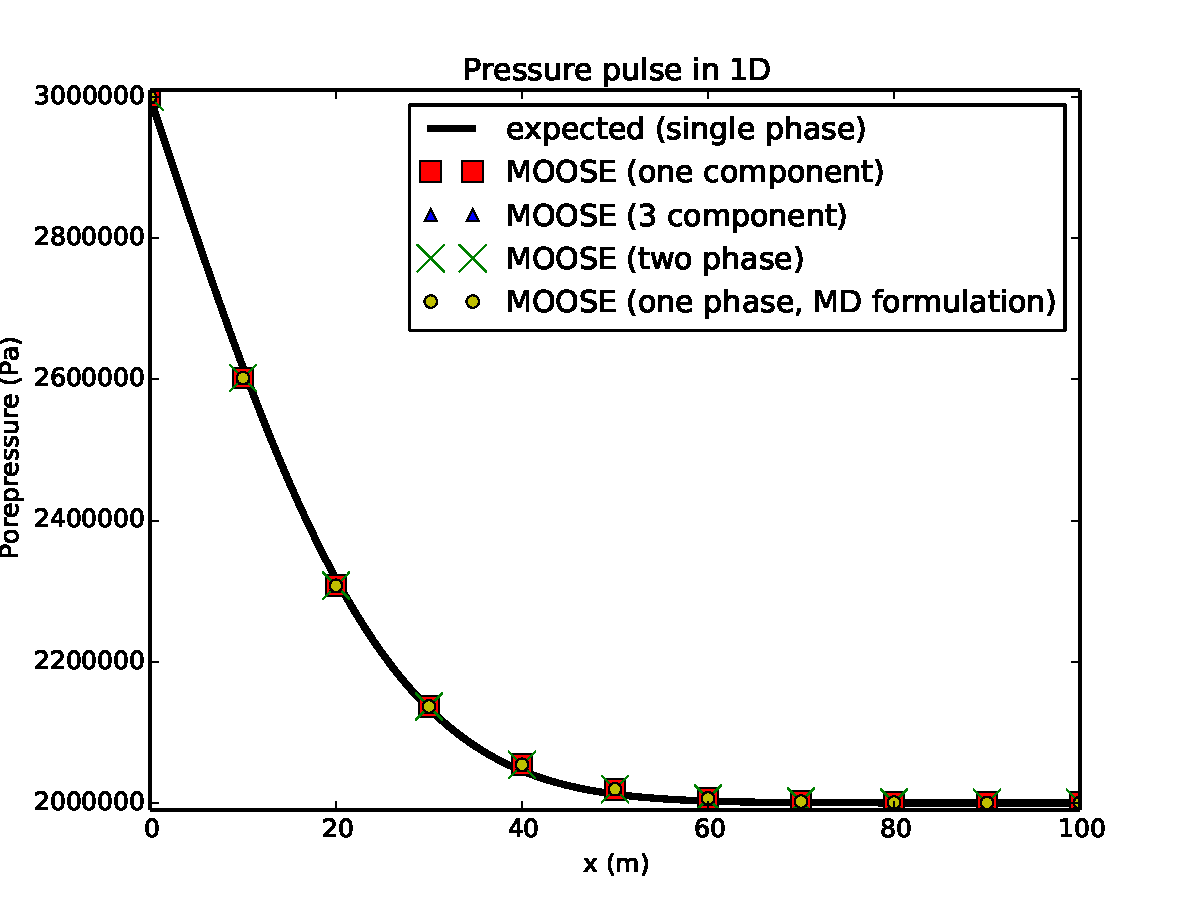
\includegraphics[width=15cm]{pressure_pulse_1d.pdf}
\caption{Comparison between the MOOSE result (in dots), and the
  exact analytic expression given by Eqn~(\ref{eqn.exact.pp}).  This
  test had 10 elements in the $x$ direction, with $0\leq x \leq
  100$\,m, and ran for a total of
  10$^4$ seconds with 10 timesteps.  The parameters were $B=2$\,GPa,
  $\kappa_{xx}=10^{-15}$\,m$^{2}$, $\mu=10^{-3}$\,Pa.s, $\phi=0.1$,
  with initial pressure $P=2$\,MPa, and applied pressure $P=3$\,MPa at
  $x=0$.  For greater spatial resolution and smaller timesteps the
  agreement increases.  Both the multi-component single-phase simulation and the
  2-phase fully-water-saturated simulation give identical results for
  the water porepressure.}
\label{pressure_pulse.fig}
\end{figure}



\end{document}

